
Một mặt bàn hình vuông có khối lượng m (trọng lượng phân bố đều) và cạnh dài a được treo bằng 4 sợi dây xích đồng nhất và có chiều dài L. Đặt hệ tọa độ có gốc đặt tại trung tâm của bàn, các sợi dây được gắn cố định vào mặt bàn tại 4 góc và các điểm có tọa độ $\left(\pm \frac{a}{2},\pm\frac{a}{2}\right)$. 
\begin{figure}[H]
    \centering
    \tikzset{every picture/.style={line width=0.75pt}} %set default line width to 0.75pt        

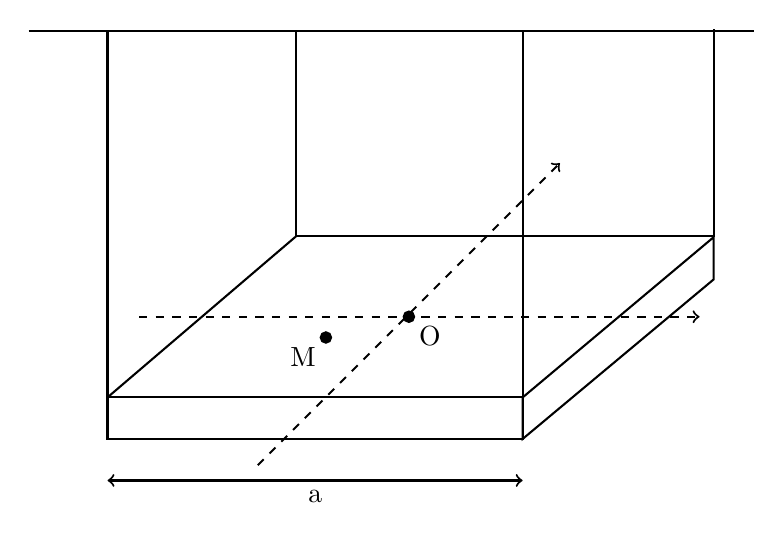
\begin{tikzpicture}[x=0.75pt,y=0.75pt,yscale=-1,xscale=1]
%uncomment if require: \path (0,429); %set diagram left start at 0, and has height of 429

%Shape: Rectangle [id:dp43479829147458826] 
\draw   (150,200) -- (350,200) -- (350,220) -- (150,220) -- cycle ;
%Shape: Rectangle [id:dp26418096458424434] 
\draw   (350,200) -- (442.03,122.78) -- (442.03,143.14) -- (350,220) -- cycle ;
%Straight Lines [id:da6303516163988201] 
\draw    (240.42,122.25) -- (442.46,122.25) ;
%Straight Lines [id:da2435007903542885] 
\draw    (149.96,200) -- (240.78,122.42) ;
%Straight Lines [id:da12397037243108167] 
\draw    (112.03,23.59) -- (461.43,23.59) ;
%Shape: Axis 2D [id:dp11255839884999319] 
%\draw [dashed] (121.01,156.7) -- (506.99,156.7)(409.6,45.33) -- (177.57,277.36) (504.99,151.7) -- (506.99,156.7) -- (494.99,161.7) (397.6,52.33) -- (409.6,45.33) -- (407.6,52.33)  ;
%Straight Lines [id:da6910540327628811] 
\draw    (150,200) -- (150,23.64) ;
%Straight Lines [id:da778712219228807] 
\draw    (241,122.34) -- (241,23.55) ;
%Straight Lines [id:da014093703911455924] 
\draw    (442,122.34) -- (442,22.35) ;
%Straight Lines [id:da13741894893199325] 
\draw    (350,200) -- (350,104.51) -- (350,23.64) ;


% Text Node

\filldraw(255.21,171.12) circle(2.5)node [anchor=north east][align=right] {M};

\draw [<->](150,240) -- (250,240)node[below]{a} -- (350,240) ;

\draw [dashed] [->] (165.23,161.12) -- (435.23,161.12);
\draw [dashed] [->] (222.42,232.62) -- (367.93,87.11);
\filldraw(295.21,161.12) circle(2.5) node [anchor=north west][align=left] {O};
\end{tikzpicture}
    \caption{}
    \label{fig:P4_01}
\end{figure}
Giả sử trọng lượng của các dây xích là không đáng kể so với trọng lượng của mặt bàn.
Bên trên mặt bàn, ta đặt một chậu cây có khối lượng M. Đối với bài này, ta coi đế của chậu cây là rất nhỏ so với mặt bàn và coi chậu là một chất điểm M.
\begin{enumerate} [label=(\alph*)]
    \item Khi chậu cây đặt đúng tại tâm bàn và đang cân bằng, giả sử dây không giãn, hãy chứng minh lực căng trong mỗi dây được tính theo công thức:
    \begin{equation}
        T = \dfrac{(m+M)g}{4}
    \end{equation}
\item 
\begin{enumerate}[label=(\roman*)]
\item Đặt chậu cây tại vị trí (x,y), hãy tìm lực căng của từng dây. Coi rằng các dây đều
tuân theo định luật Hooke: $T = k \cdot\Delta{x}$ với $\Delta{x}$ là độ dãn của dây. Cho rằng hệ số đàn hồi k của dây là rất lớn, giới hạn đàn hồi của dây là đủ nhỏ để độ nghiêng của mặt bàn là không đáng kể.
\item Khi không chịu bắt cứ lực căng nào, dây sẽ bị chùng, tìm những vị trí  đặt chậu cây M trên bàn thoả mãn.
\item Dây sẽ bị đứt khi $\Delta{x}>\Delta{l_0}$, tìm quỹ tích các vị trí đặt chậu cây để hệ cân bằng.
\end{enumerate}
\end{enumerate}